\documentclass[12pt]{book}

\usepackage{amssymb}
\usepackage{amsmath}
\usepackage{amsthm}
\usepackage{amsfonts}
\usepackage[spanish]{babel}
\usepackage[utf8]{inputenc}
\usepackage[T1]{fontenc}
\usepackage{graphicx}
\usepackage[figuresright]{rotating}
\usepackage{subfigure}
\usepackage{epstopdf}
\usepackage{float}
\usepackage{natbib}
\usepackage[skip=10pt,labelfont=bf,labelsep=period]{caption}
\usepackage[paperwidth=215mm,paperheight=280mm,left=40mm,top=40mm,textwidth=150mm,textheight=215mm]{geometry} 
\usepackage{fancybox}
\usepackage{fancyhdr}
\usepackage{enumerate}
\usepackage{url} 
\usepackage{newtxtext,newtxmath}
\usepackage{bm}

\theoremstyle{definition}
\newtheorem{theorem}{Teorema}[chapter]
\newtheorem{example}[theorem]{Ejemplo}
\newtheorem{proposition}[theorem]{Proposición}
\newtheorem{definition}[theorem]{Definición}
\newtheorem{Lem}[theorem]{Lema}
\newtheorem{Cor}[theorem]{Corolario}
\newtheorem{remark}[theorem]{Observación}
\newtheorem{note}[theorem]{Nota}
\DeclareMathOperator{\sign}{sign}
\DeclareMathOperator*{\argmax}{\arg\,\max}
\usepackage{mathtools}
\newcommand{\Op}[3]{\prescript{}{#2}{#1}^{#3}_{t}}
\newcommand{\OpFull}[5]{\prescript{#1}{#2}{#3}^{#4}_{#5}}
\spanishdecimal{.}

%% Comandos basicos en el texto
%% ==================================================================
\newcommand{\set}[2]{\{#1\nonscript\;\vert\allowbreak\nonscript\:\mathopen{}#2\}}
\usepackage{dsfont}

\begin{document}
\begin{titlepage}

	\vfill

	{\LARGE Trabajo en teoría de Gráficas}\\[2cm]

	\vfill
\end{titlepage}
\chapter{Gráficas clan críticas y gráficas de clanes}
\section{Definiciones}
En este trabajo se consideran gráficas simples, finitas, sin lazos y conexas.
\begin{definition}
Una gráfica $G$ consta de dos conjuntos $G=(V,E)$, donde $V$ es un conjunto cualquiera y $E\subset \set{\left\{u,v\right\}\subset V}{u\neq v}$. El conjunto $V$ o $V(G)$ es llamado conjunto de vértices de la gráfica $G$. Los elementos de $E$ o $E(G)$ se llaman aristas de la gráfica $G$.
\end{definition}

\begin{definition}
Sea $G=(V,E)$ una gráfica. Si $u,v\in V(G)$ son tal que $\left\{u,v\right\}\in E(G)$, decimos que $u$ y $v$ son adyacentes. Se denota tal adyacencia por $u\sim v$.
\end{definition}

\begin{definition}[\citealt{Harary:1969}]
Un camino de una gráfica $G$, es una sucesión de vértices $u_0,u_1,\dots,u_{n-1},u_n$, tales que existe una adyacencia de cada uno de los vértices con el vértice inmediato anterior y el inmediato siguiente. Se suele denotar tal camino como $u_0u_n-$camino.
\end{definition}

\begin{definition}[\citealt{Harary:1969}]
Una gráfica es conexa si cada par de vértices está unido por un camino.
\end{definition}
Se define una gráfica disconexa, a la gráfica que no es conexa.

\begin{definition}
Sea $G$ una gráfica. Un ciclo de G es un $uv-$camino que es cerrado, es decir, que se satisface que $u=v$.
\end{definition}

\begin{definition}[\citealt{Harary:1969}]
Una gráfica es acíclica si no tiene ciclos. Un árbol es una gráfica acíclica conexa. 
\end{definition}

\begin{definition}
Sea $G$ una gráfica. Una subgráfica de $G$ es una gráfica $H$ tal que $V(H)\subset V(G)$ y $E(H)\subset E(G)$.
\end{definition}

\begin{definition}
Sea $G$ una gráfica y $H$ una subgráfica de $G$. $H$ es una subgráfica inducida si para todo $u,v\in V(H)$ tales que $u\sim v$ en $G$ entonces $u\sim v$ en $H$.
\end{definition}

Se entiende que una subgráfica completa $H_n$ tiene cada par de sus $n$ vértices adyacentes. Dicha gráfica completa es maximal si no existe otro vértice en la gráfica tal que forme una completa más grande. Lo anterior da paso a la siguiente definición.

\begin{definition}[\citealt{Harary:1969}]
Un clan de $G$ es una subgráfica completa maximal. 
\end{definition}

\begin{definition}[\citealt{Roberts:1971}]
Dado $G$ una gráfica, sean $q_1, q_2, \dots, q_n $ sus clanes. Definimos $H'$ mediante $ V(H') = \{q_1, q_2, \dots, q_n\}$ y $\left\{q_i, q_j\right\}\in E(H')$ si y solo si $i \neq j$ y $q_i \cap q_j \neq \emptyset$.  
Entonces, llamamos a $H'$ como la gráfica de clanes de $G$ y escribimos $H'=K(G)$.
\end{definition}

\begin{definition}[\citealt{Alcon:2006}]
Sea $G$ una gráfica y $v \in V(G)$. Como es habitual, $G-v$ denota la gráfica inducida por $V(G)\setminus \{v\}$.  
\end{definition}

\begin{definition}[\citealt{Escalante:1974}]
El vértice $v$ es clan crítico si $K(G)\neq K(G-v)$. Una gráfica $G$ es clan crítica si cada uno de sus vértices es crítico.
\end{definition}



\section{Resultados}

En el siguiente teorema se consideran las gráficas $G(4,3,3)$, que denota a la gráfica con 4 vértices, 3 aristas, número 3; y la gráfica $G(5,7,1)$, que denota la gráfica de 5 vértices, 7 aristas, número 1. Dichas gráficas son extraídas del apéndice de gráficas en \cite{Harary:1969}, ver la figura~\ref{F1}.

\begin{figure}[!htbp]
	\centering
	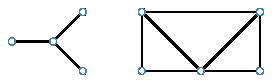
\includegraphics[scale=1.2]{Fig0.pdf}
	\caption{Esquema de las gráficas $G(4,3,3)$ (izquierda) y $G(5,7,1)$ (derecha).\label{F1}}
\end{figure}

\begin{theorem}
	Sea $G$ una gráfica clan crítica tal que su gráfica de clanes es $K_3$, entonces $G$ es la gráfica $G(4,3,3)$ ó $G(5,7,1)$.
\end{theorem}
\begin{proof}
Sea $G$ una gráfica clan crítica tal que $K(G)=K_3$. Al ser $K(G)=K_3$ entonces existen $q_1,q_2,q_3$ clanes de $G$, representados como los vértices de $K_3$. Cada par de clanes se interseca en al menos un vértice de $G$, es decir
\begin{equation*}
q_i\cap q_j\neq \emptyset, \quad \forall i,j\in\{1,2,3\},\quad i\neq j.
\end{equation*}
A continuación se muestra que existe un vértice $u_1$ de $G$, en el que se intersecan necesariamente los tres clanes de $G$, es decir $\{u_1\}\subset q_1\cap q_2 \cap q_3$. 

Supongamos que no existe un vértice $u_1$ que pertenezca simultáneamente a los tres clanes, es decir  $q_1\cap q_2 \cap q_3=\emptyset$. Bajo este supuesto, cada intersección $q_i\cap q_j$, $i\neq j$, contiene al menos un vértice, pero no hay un vértice común a todos. Sea $x_{ij}\in q_{i}\cap q_{j}$. Entonces $\{x_{12},x_{13},x_{23}\}$ forman una completa que se puede extender a un clan $q$. El clan $q$ es diferente de $q_{1},q_{2},q_{3}$ (pues, por ejemplo, $x_{23}\in q$ pero $x_{23}\not\in q_{1}$ por la condición de que $q_{1}\cap q_{2}\cap q_{3}=\emptyset$), lo cual contradice que $G$ sólo tenía los tres clanes $q_{1},q_{2},q_{3}$. 
Por lo tanto, necesariamente debe existir al menos un vértice $u_1$ tal que
\begin{equation*}
\{u_1\}\subset q_1\cap q_2 \cap q_3.
\end{equation*}
Para mostrar una igualdad estricta entre dichos conjuntos se sigue el siguiente argumento.

Supongamos existen $n$ vértices en dicha intersección de los tres clanes, con $n>1$. Con lo cual estos $n$ vértices pertenecen a cada uno de los clanes, es decir $\{u_1, \dots , u_n\} \subset q_i$ con $i\in\{1,2,3\}$. Sin embargo, esto implicaría que dichos vértices son adyacentes entre sí, formando un clan en $G$, lo que contradice el hecho de que solo existen tres clanes en $G$, por lo tanto se satisface 
\begin{equation*}
	\{u_1\}=q_1\cap q_2 \cap q_3.
\end{equation*}

En busca de saber que gráfica es $G$, consideramos las intersecciones que pueden tener los clanes, con lo cual, resultan los siguientes casos a tratar, los cuales están considerando el hecho de la existencia del vértice $u_1$.
\begin{itemize}
\item Caso 1. 
Los clanes de $G$ se intersecan únicamente en el vértice $u_1$, es decir $q_1\cap q_2\cap q_3=\left\{u_1\right\}$, $(q_1\cap q_3)\setminus q_2=\emptyset  \text{, }(q_2\cap q_3)\setminus q_1=\emptyset$ y $(q_1\cap q_2)\setminus q_3=\emptyset$, como se muestra en la figura~\ref{F2}.

\begin{figure}[!htbp]
	\centering
	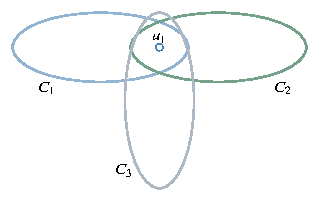
\includegraphics[scale=1.2]{Fig1.pdf}
	\caption{Esquema de los clanes de la gráfica $G$ correspondiente al caso 1.\label{F2}}
\end{figure}

De primera instancia, los tres clanes pueden estar constituidos por $n$ vértices (no necesariamente la misma $n$ para cada uno de los clanes), sin embargo, de considerar un $n>2$, la gráfica $G$ no cumpliría la condición de ser clan crítica, pues resultaría que $K(G)=K(G-\hat{u})$, para cualquier $\hat{u}\in V(q_i)$, $i\in\{1,2,3\}$ y $\hat{u}\neq u_1$. Por lo tanto cada clan consta únicamente de dos vértices, con lo cual la gráfica $G=G(4,3,3)$.

\item Caso 2.
Existe una intersección dos a dos entre los clanes, de más de un vértice, considerando el vértice $u_1$. Sin pérdida de generalidad, supongamos que el clan $q_3$ interseca al clan $q_1$ en un vértice $u_2\in V(G)$, así como a $q_2$ en un vértice $u_3\in V(G)$, esto es 
\begin{equation}\label{E1.1}
\left\{u_2\right\}=(q_1\cap q_3)\setminus q_2 \quad \text{y} \quad \left\{u_3\right\}=(q_2\cap q_3)\setminus q_1.
\end{equation}
Como se muestra en la figura~\ref{F3}.

El argumento de que no exista más de un vértice en cada uno de los conjuntos en \eqref{E1.1}, es análogo al razonamiento expuesto al inicio de la prueba, es decir, de existir más de un vértice, éstos formarían un nuevo clan de $G$, lo que contradice la hipótesis de que $K(G)=K_3$, por lo tanto, es correcta la expresión \eqref{E1.1}.

\begin{figure}[!htbp]
	\centering
	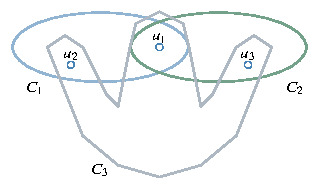
\includegraphics[scale=1.2]{Fig2.pdf}
	\caption{Esquema de los clanes de la gráfica $G$ correspondiente al caso 2.\label{F3}}
\end{figure}

A continuación demostraremos que los clanes $q_1$ y $q_2$ no pueden ser tales que están constituidos únicamente de dos vértices. 
Supongamos que $|q_1|=2$ y $|q_2|=2$, con lo cual $\left\{\left\{u_2,u_1\right\},\left\{u_1,u_3\right\},\left\{u_2,u_3\right\}\right\}\subset E(G)$, de esta manera, se formaría un nuevo clan distinto a $q_1,q_2$ y $q_3$, lo que contradiría la hipótesis de $K(G)=K_3$, pues existirían cuatro vértices en $K(G)$ y no tres. Como los clanes $q_1$ y $q_2$ no pueden tener solo dos vértices, deben tener al menos tres y no más pues se busca que la gráfica sea clan crítica, con lo cual se buscan clanes con menor cantidad de vértices posibles.
Siguiendo este razonamiento, se puede concluir que $|q_1|=|q_2|=|q_3|=3$, lo que da lugar a la gráfica $G=G(5,7,1)$.


\item Caso 3.
Los clanes de $G$ se intersecan en el vértice $u_1$ y sólo existe otra intersección entre dos de estos clanes. Sin pérdida de generalidad, supongamos que los clanes $q_1$ y $q_3$ se intersecan en un vértice $u_2$ de $G$ y $(q_2\cap q_3)\setminus q_1=\emptyset $, como se muestra en la figura~\ref{F4}.

\begin{figure}[!htbp]
	\centering
	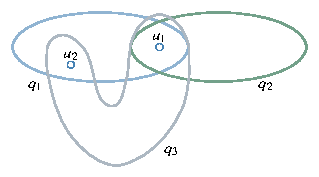
\includegraphics[scale=1.2]{Fig3.pdf}
	\caption{Esquema de los clanes de la gráfica $G$ correspondiente al caso 3.\label{F4}}
\end{figure}

Veamos que los clanes $q_1,q_3$ están constituidos únicamente por tres vértices. Pues si alguno de estos clanes tuviera menos de tres vértices, entonces existiría un vértice $\hat{u}$ en $q_1$ ó $q_3$ cuya eliminación no cambiaría la estructura de $K(G)$, lo que contradice la definición de clan crítica.

Por otro lado, consideremos $u_3\in V(q_3)$ tal que $u_3\neq u_1,u_2$. El clan $q_2$ debe estar constituido de más de dos vértices, pues de no ser así, consideremos un nuevo vértice $\hat{u}\neq u_1$ en $q_2$, ver figura~\ref{F5}.

\begin{figure}[!htbp]
	\centering
	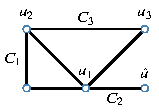
\includegraphics[scale=1.2]{Fig4.pdf}
	\caption{Esquema de los vértices y clanes de la gráfica $G$ correspondiente al caso 3, suponiendo que $q_2$ cuenta únicamente con dos vértices.\label{F5}}
\end{figure}

En tal caso se cumple que $K(G-u_2)=K(G)$, situación que no es válida. Con lo cual $|q_2|>2$ y se consideran los siguientes dos casos.
\begin{itemize}
\item Caso 3.1.
El vértice $u_3\notin V(q_2)$, entonces para todo $\overline{u}\in V(q_2)\setminus\{u_1\}$ se tiene que $K(G-\overline{u})=K(G)$, lo que implica que este caso no es posible, pues la eliminación de cualquier vértice de $q_2$, excepto $u_1$, no provoca un cambio en la estructura de $K_3$, lo que contradiría la hipótesis de clan crítica.

\item Caso 3.2.
El vértice $u_3\in V(q_2)$. Este caso se reduce al caso 2, con lo cual $G=G(5,7,1)$.
\end{itemize}
\end{itemize}
Resulta entonces que $G$ es la gráfica $G(4,3,3)$ ó $G(5,7,1)$.
\end{proof}


En el siguiente teorema se consideran las gráficas $G(3)$ y $G(4)$ que denotan el camino compuesto de tres y cuatro vértices respectivamente, ver figura~\ref{F6}.

\begin{figure}[!htbp]
	\centering
	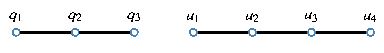
\includegraphics[scale=1.2]{Fig5.pdf}
	\caption{Esquema de las gráficas $G(3)$ (izquierda) y $G(4)$ (derecha), con sus respectivas etiquetas de acuerdo a sus vértices.\label{F6}}
\end{figure}

\begin{theorem}\label{T1.12}
Sea $G$ una gráfica clan crítica tal que su gráfica de clanes es $G(3)$, entonces $G$ es la gráfica $G(4)$.
\end{theorem}

\begin{proof}
Sea $G$ una gráfica clan crítica tal que $K(G)=G(3)$. La igualdad anterior implica directamente que existen únicamente tres clanes $q_1$, $q_2$ y $q_3$ tal que $q_1\cap q_3=\emptyset$. Dichos clanes están representados como los vértices de $G(3)$, ver figura~\ref{F6}.
Notemos que el clan $q_2$ tiene intersección no vacía con $q_1$ y $q_3$. A continuación se muestra un argumento con el cual es posible afirmar que en las intersecciones $q_1\cap q_2$ y $q_3\cap q_2$ constan únicamente de un vértice $u_2$ y $u_3$ de $G$, respectivamente.

Supongamos que existen $n$ vértices $\{v_1,\dots,v_n\}$ en $q_1\cap q_2$ con $n>1$, con lo cual se cumplen las siguientes contenciones $\{v_1,\dots,v_n\}\subset q_1 $ y $\{v_1,\dots,v_n\}\subset q_2$, lo que implica que los vértices $\{v_1,\dots,v_n\}$ son mutuamente adyacentes entre sí, lo que formaría un nuevo clan de $G$, de esta manera no se cumpliría que su gráfica de clanes fuese $G(3)$, pues tendría más de tres vértices su gráfica de clanes, esta contradicción viene del hecho de suponer la existencia de $n$ vértices en $q_1\cap q_2$ con $n>1$, con lo cual tiene que ser $n=1$. Por lo tanto se satisface que 
\begin{equation*}
\{u_2\}=q_1\cap q_2.
\end{equation*}
Con un razonamiento análogo, se demuestra que de igual manera se satisface que 
\begin{equation*}
	\{u_3\}=q_3\cap q_2.
\end{equation*}

Por otra parte, lo que sigue es un razonamiento que demuestra que el clan $q_1$ está constituido de solo dos vértices, el ya mencionado $u_2$ y uno más en G; de igual manera el clan $q_3$ está constituido por el mencionado vértice $u_3$ y uno más en $G$. Demostraremos estos hechos para el caso del clan $q_1$, pues como anteriormente sucedió, el caso para la demostración del clan $q_3$ resultará análogo a la prueba del $q_1$. 


Así pues, consideremos que el clan $q_1$ está constituido por más de dos vértices, digamos $V(q_1)=\{v_1,\dots v_n\}$. Por ser un clan $q_1$, resulta que $q_1-v_i$ es un clan también, para cualquier $i\in \{1,\dots,n\}$, con lo cual, cualquier eliminación de $V(q_1)$, excepto $u_2$, no provoca un cambio en la estructura de su gráfica de clanes, lo que contradiría la hipótesis de clan crítica. Por lo tanto se requiere que $q_1$ tenga la menor cantidad de vértices posibles y que siga siendo un clan, por lo tanto sólo consta de dos vértices, $u_2$ y uno más llamemosle $u_1$. De esta manera, también $q_3$ consta únicamente de dos vértices, $u_3$ y uno más, llamemosle $u_4$.

De acuerdo con el razonamiento planteado anteriormente, el clan $q_2$ también debe de constar únicamente de dos vértices, pues de ser más, se contradice la hipótesis de ser $G$ clan crítica. Con lo cual, se puede concluir que $G$ es un camino de cuatro vértices, es decir, $G=G(4)$.
\end{proof}

El siguiente teorema es una generalización del teorema anterior, se consideran las gráficas $G(n-1)$ y $G(n)$, que denotan el camino compuesto por $n-1$ vértices y $n$ vértices, respectivamente. Ver figura~\ref{F7}.

\begin{figure}[!htbp]
	\centering
	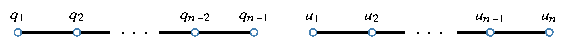
\includegraphics[scale=1.2]{Fig6.pdf}
	\caption{Esquema de las gráficas $G(n-1)$ (izquierda) y $G(n)$ (derecha), con sus respectivas etiquetas de acuerdo a sus vértices.\label{F7}}
\end{figure}

\begin{theorem}
Sea $G$ una gráfica clan crítica tal que su gráfica de clanes es $G(n-1)$, entonces $G$ es la gráfica $G(n)$.
\end{theorem}

\begin{proof}
Por hipótesis $K(G)=G(n-1)$, lo que implica que en $G$ existen $n-1$ clanes diferentes, que satisfacen $q_{k-1}\cap q_{k+1}=\emptyset$ para $k\in\{2,\dots n-2\}$; que representan los vértices de $G(n-1)$, como se muestra en la figura~\ref{F7} (izquierda).

Notemos que cada vértice en $G(n-1)$, que representa un clan de $G$, es adyacente con el vértice inmediato anterior y el inmediato siguiente. En el caso del primer vértice, adyacente con el inmediato siguiente; y en el caso del último vértice, adyacente con el inmediato anterior. Esto es que las intersecciones $q_1\cap q_2$, $q_2\cap q_3$, $\dots$ , $q_{n-3}\cap q_{n-2}$, $q_{n-2}\cap q_{n-1}$ son no vacías. Utilizando el mismo razonamiento expuesto en el teorema~\ref{T1.12}, se muestra que cada una de estas intersecciones es un único vértice, es decir
\begin{equation*}
\begin{aligned}
q_1\cap q_2 &= \{u_2\} \\
q_2\cap q_3 &= \{u_3\} \\
\vdots \\
q_{n-3}\cap q_{n-2} &= \{u_{n-2}\} \\
q_{n-2}\cap q_{n-1} &= \{u_{n-1}\}.
\end{aligned}
\end{equation*}

Por otra parte, de igual manera como se hizo en el teorema~\ref{T1.12}, se demostrará que el clan $q_1$ está constituido de solo dos vértices, el ya mencionado $u_2$ y uno más en G; de igual manera el clan $q_{n-1}$ está constituido por el mencionado vértice $u_{n-1}$ y uno más en $G$. Demostraremos estos hechos para el caso del clan $q_1$, pues el caso para la demostración del clan $q_{n-1}$ resultará análogo a la prueba del $q_1$. 

Consideremos que el clan $q_1$ está constituido por más de dos vértices, digamos $V(q_1)=\{v_1,\dots v_n\}$. Por ser un clan $q_1$, resulta que $q_1-v_i$ es un clan también, para cualquier $i\in \{1,\dots,n\}$, con lo cual, cualquier eliminación de $V(q_1)$, excepto $u_2$, no provoca un cambio en la estructura de su gráfica de clanes, lo que contradiría la hipótesis de clan crítica, por lo tanto sólo consta de dos vértices, $u_2$ y uno más llamemosle $u_1$, pues de esta manera la eliminación de dicho vétice $u_1$ provoca un cambio en la estructura de la gráfica de clanes de $G$, cumpliendo las hipótesis de ser clan crítica. 
De esta manera, también $q_{n-1}$ consta únicamente de dos vértices, $u_{n-1}$ y uno más, llamemosle $u_n$.

De acuerdo con el razonamiento planteado anteriormente, los clanes $q_2$, $q_3$, $\dots$ , $q_{n-3}$, $q_{n-2}$ también deben de constar únicamente de dos vértices, pues de ser más, se contradice la hipótesis de ser $G$ clan crítica, como se mostró. Con lo cual, se puede concluir que $G$ es un camino de $n$ vértices, es decir, $G=G(n)$.
\end{proof}

El siguiente teorema hace referencia la relación que existe entre la gráfica $G(6,6,18)$ y el árbol $T(4,2)$, extraídos del apéndice de gráficas y de diagramas de árbol en \cite{Harary:1969}, respectivamente. Dichas gráficas pueden verse en la figura~\ref{F8}

\begin{figure}[!htbp]
	\centering
	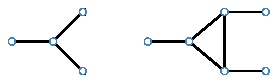
\includegraphics[scale=1.2]{Fig7.pdf}
	\caption{Esquema de las gráficas $T(4,2)$ (izquierda), con las etiquetas de sus vértices, y $G(6,6,18)$ (derecha).\label{F8}}
\end{figure}

\begin{theorem}
Sea $G$ una gráfica clan crítica tal que su gráfica de clanes es $T(4,2)$, entonces $G$ es la gráfica $G(6,6,18)$.
\end{theorem}

\begin{proof}
Sea $G$ una gráfica clan crítica tal que su gráfica de clanes es $T(4,2)$. Con lo cual, la gráfica $G$ debe tener cuatro clanes $q_1$, $q_2$, $q_3$ y $q_4$, representados como los vértices de $T(4,2)$, como se muestra en la figura~\ref{F8}. Por las características de la gráfica de clanes de $G$, los clanes satisfacen que $q_1\cap q_3=\emptyset$, $q_1\cap q_4=\emptyset$ y $q_3\cap q_4=\emptyset$, además el clan $q_1$ tiene intersección no vacía con todos los demás.

El siguiente razonamiento concluye que las intersecciones que existen entre $q_1$ con los demás clanes consta de un sólo vértice. Resulta que la prueba para cualquiera de estos clanes con $q_1$ es análoga, con lo cual se demostrará en el caso cuando se considera la intersección $q_1\cap q_2$.

Supongamos que en $q_1\cap q_2=\{v_1, \dots ,v_n\}$, es decir, existen $n$ vértices con $n>1$. Con lo cual se satisface $\{v_1, \dots ,v_n\}\subset q_1$ y $\{v_1, \dots ,v_n\}\subset q_2$, lo que satisface que $\{v_1, \dots ,v_n\}$ son mutuamente adyacentes, forman un clan de $G$ distinto a los cuatro ya contemplados, lo que contradiría la hipótesis de que $K(G)=T(4,2)$, pues existirían al menos cinco clanes. Dicha contradicción viene del hecho de suponer que $n>1$, con lo cual $n=1$, $q_1\cap q_2$ consta únicamente de un vértice, es decir
\begin{equation*}
q_1\cap q_2= \{u_2\}.
\end{equation*}
Por lo tanto, de igual manera se satisface que 
\begin{equation*}
\begin{aligned}
q_3\cap q_2 &= \{u_3\}, \\
q_4\cap q_2 &= \{u_4\}.
\end{aligned}
\end{equation*}

Los vértices $u_2$, $u_3$ y $u_4$, son distintos, pues de no serlo, las propiedades de $K(G)$ $q_1\cap q_3=\emptyset$, $q_1\cap q_4=\emptyset$ y $q_3\cap q_4=\emptyset$ no se satisfacerían. Este hecho implica que en $q_2$ existen al menos tres clanes, y enrealidad, existen solo esos tres vértices, pues de existir más, no se cumpliría que $G$ fuese clan crítica, pues cualquier eliminación de vértices, que no sea $u_2$, $u_3$, $u_4$; no cambiaría la estructura de su gráfica de clanes.
De manera análoga, se demostrará que $q_1$, $q_3$ y $q_4$ constan únicamente de dos vértices. Supongamos que $V(q_1)=\{v_1, \dots ,v_n\}$ con $n>2$. Al ser un clan $q_1$, se cumpliría la igualdad $K(G)=K(G-v_i)$ con $v_i\in V(q_1)$ y $v_i\neq u_2$, lo que implicaría que $G$ es no clan crítica. La contradicción se produce al suponer que $n>2$, por lo tanto $n=2$. Como se dijo, de manera análoga se demuestra que $q_3$ y $q_4$ constan únicamente de dos vértices.

Por lo tanto la gráfica $G$ correspondiente es la gráfica $G(6,6,18)$.
\end{proof}

El siguiente teorema considera el árbol $T(5,3)$ expuesto en el apéndice de diagramas de árbol en \cite{Harary:1969} y la gráfica $G(8,10)$, que representa la gráfica de ocho vértices y diez aristas, formando un ciclo de cuatro vértices. Los esquemas de dichas gráficas se pueden ver en la figura~\ref{F9}.

\begin{figure}[!htbp]
	\centering
	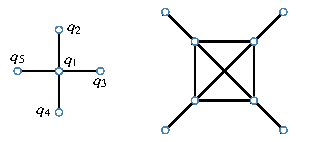
\includegraphics[scale=1.2]{Fig9.pdf}
	\caption{Esquema de las gráficas $T(5,3)$ (izquierda) y $G(8,10)$ (derecha).\label{F9}}
\end{figure}

\begin{theorem}
Sea $G$ una gráfica clan crítica tal que su gráfica de clanes es $T(5,3)$, entonces $G$ es la gráfica $G(8,10)$.
\end{theorem}




\bibliography{Ref}
\bibliographystyle{apalike}

\end{document}
